\documentclass[a4paper]{article}

\usepackage{hyperref, amsmath, graphicx, float, blindtext} % for dummy text
\graphicspath{ {./images/} }
\title{Attention is all you need}
\author{Shubham Gupta}

\begin{document}
\maketitle
\section{Introduction}
\begin{itemize}
    \item This paper review is following the blog from Jay Alammar's blog on the \textbf{Illustrated Transformer}. The blog can be found \href{https://jalammar.github.io/illustrated-transformer/}{here}.  
\end{itemize}
\section{Paper Introduction}
\begin{itemize}
    \item New architecture based solely on attention mechanisms called \textbf{Transformer}. Gets rids of recurrent and convolution networks completely.  
    \item Generally, RNN used to seq-to-seq tasks such as translation, language modelling, etc.
    \item Transformer allows for significant parallelization and relies only on attention.
\end{itemize}
\section{Background}
\begin{itemize}
    \item \textit{Self attention} Attention to different positions of a sequence in order to compute a representation of the sequence.
\end{itemize}
\section{Model Architecture}
\begin{itemize}
    \item Transformer uses the following:
    \begin{itemize}
        \item Encoder decode mechanism
        \item Stacked self attention
        \item Point wise fully connected layer for encoder and decoder
    \end{itemize}
    \begin{figure}[H]
        \centering
        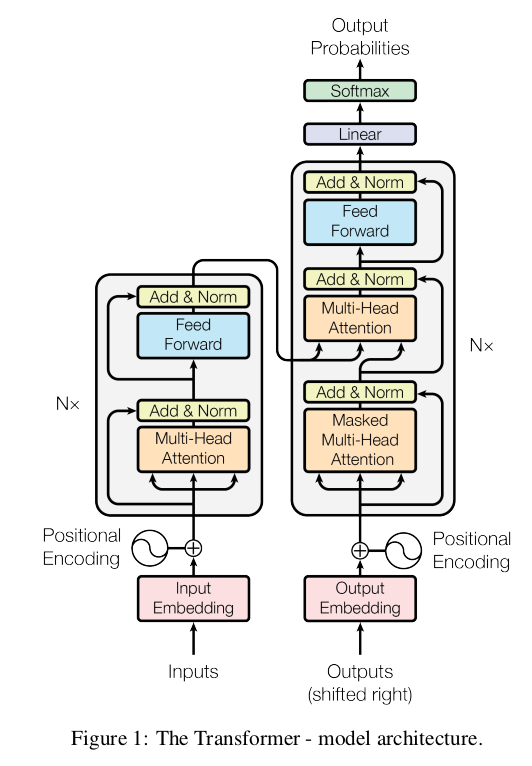
\includegraphics[width=0.8\textwidth]{transformer}
        \caption{transformer}
        \label{fig:transformer}
    \end{figure}
\end{itemize}
\subsection{Encoder and decoder stacks}
\begin{itemize}
    \item \textbf{Encoder}: 6 identical layers. 2 sub layers per layer
    \item \textit{First}: multi-head self attention mechanism
    \item \textit{Second}: Fully connected feed forward network
    \item Apply residual connection for each of the two laters
    \item Apply layer normalization
    \item \textbf{Decoder}: 6 identical layers. 2 sub layers as above + 1 more which performs multi-head attention over output of encoder stack 
    \item Resodual locks around all 3 sub layers
    \item Layer normalization
    \item Modify self-attention sub layer to prevent positions from attending to subsequent positions. Ensures that \textit{i} output depends only on words before \textit{i}.
\end{itemize}
\subsection{Attention}
\begin{itemize}
    \item 3 vectors: Query(Q), Key(K) and Value(V)
    \item Output = Weighted sum of values. Weights assigned as a function of query with key.
    \item Scaled dot-product attention and multi-head attention
    \begin{figure}[H]
        \centering
        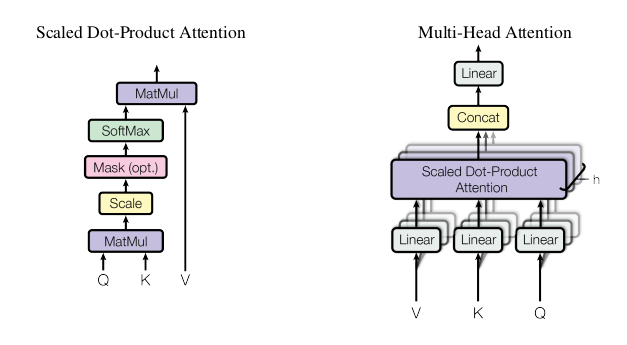
\includegraphics[width=0.8\textwidth]{attention_types}
        \caption{Types of attention}
        \label{fig:attention_types}
    \end{figure}
    \item Attention is calculated as:
    \begin{equation}
    \begin{split}
        Attention(Q,K,V) = softmax(\frac{QK6T}{\sqrt{d_k}})V
    \end{split}
    \end{equation}
    \item Dot product attention is \textbf{faster and more space-efficient} than additive attention. 
\end{itemize}
\subsection{Multi head attention}
\begin{itemize}
    \item Using multile q, k and v vectors. Get the final output, concatenate them and get another final projection $d_{v}$.
    \begin{equation}
    \begin{split}
        MultiHead(Q,K,V) = Concat(head_1,...,head_h)W^O
        were head_i = Attention(QW_{i}^{Q}, KW_{i}^{K},VW_{i}^{V})
    \end{split}
    \end{equation}
\item $d_{k} = d_{v} = d_{model}/h = 64$
\end{itemize}
\subsection{Applications of attention}
\begin{itemize}
    \item \textbf{Encoder-decoder attention}: Q from previours decoder, K and V from output of decoder. Attend to all positions in the input sequence. 
    \item \textbf{Encoder}: Self attentnion laters. Q,K and V from output of previous layer in the encoder. Some talk about leftward flow, didn't really understand this bit.  Will come back to this in sometime.
\end{itemize}
\subsection{Position-wise Feed-Forward Networks}
\begin{itemize}
    \item Each layer contains feed-forward network.
    \begin{equation}
    \begin{split}
        FFN(x) = max(o, xW_1,+ b_1)W_2 + b_2
    \end{split}
    \end{equation}
\end{itemize}
\subsection{Embeddings and Softmax}
\begin{itemize}
    \item Convert input and output string to vectors of dim $d_{model}$
    \item Share weight matrix between two embedding layers and the pre-softmaax linear transformation
\end{itemize}
\subsection{Positional Encoding}
\begin{itemize}
    \item Encode positions of the tokens for the input and output.
    \item Same vector size i.e $d_{model}$
    \begin{equation}
    \begin{split}
        PE_{(pos, 2i)} = sin(pos/10000^{2i/d_{model}}
        PE_{(pos, 2i+1)} = cos(pos/10000^{2i/d_{model}}
    \end{split}
    \end{equation}
    \item Might allow approximation of longer sequence lenghts than seen in the training set
\end{itemize}
\subsection{Why self attentnion?}
\begin{itemize}
    \item Total computational complexity per layer
    \item Parallel Computation
    \item Path length between long-range dependencies in the network.
\end{itemize}
\section{Training}
\subsection{Optimizer}
\begin{itemize}
    \item Use Adam. Vary learning rate according to formula: $lrate = d_{model}^{-0.5} . min(step_num^{-0.5}, step_num . warmupsteps^{-1.5})$
    \item Increase LR for warmup steps, then decrease propotionally to inverse square root of step number. Warmup steps = 4000
\end{itemize}
\subsection{Regularization}
\begin{itemize}
    \item \textbf{Residual Dropout} 
    \item \textbf{Label Smoothing}: Instead of using 0 and 1 as class labels, allow for some uncertainity in the prediction, and use values like 0.1 and 0.9 for the classes 
\end{itemize}
\section{Conclusion}
\begin{itemize}
    \item This was the first model based entirely on attention. It acheived SOTA results on Machine Translation and English contituency parsing.
    \item Admittedly, there are still a lot of bits I don't really understand. Specially around self attention. I will give this paper another read after going through Jay Alammar's blog.
\end{itemize}
\end{document}
